% Options for packages loaded elsewhere
\PassOptionsToPackage{unicode}{hyperref}
\PassOptionsToPackage{hyphens}{url}
\PassOptionsToPackage{dvipsnames,svgnames,x11names}{xcolor}
%
\documentclass[
  12pt,
  a4paper,
]{article}

\usepackage{amsmath,amssymb}
\usepackage{iftex}
\ifPDFTeX
  \usepackage[T1]{fontenc}
  \usepackage[utf8]{inputenc}
  \usepackage{textcomp} % provide euro and other symbols
\else % if luatex or xetex
  \usepackage{unicode-math}
  \defaultfontfeatures{Scale=MatchLowercase}
  \defaultfontfeatures[\rmfamily]{Ligatures=TeX,Scale=1}
\fi
\usepackage{lmodern}
\ifPDFTeX\else  
    % xetex/luatex font selection
\fi
% Use upquote if available, for straight quotes in verbatim environments
\IfFileExists{upquote.sty}{\usepackage{upquote}}{}
\IfFileExists{microtype.sty}{% use microtype if available
  \usepackage[]{microtype}
  \UseMicrotypeSet[protrusion]{basicmath} % disable protrusion for tt fonts
}{}
\makeatletter
\@ifundefined{KOMAClassName}{% if non-KOMA class
  \IfFileExists{parskip.sty}{%
    \usepackage{parskip}
  }{% else
    \setlength{\parindent}{0pt}
    \setlength{\parskip}{6pt plus 2pt minus 1pt}}
}{% if KOMA class
  \KOMAoptions{parskip=half}}
\makeatother
\usepackage{xcolor}
\usepackage[margin=1in]{geometry}
\setlength{\emergencystretch}{3em} % prevent overfull lines
\setcounter{secnumdepth}{5}
% Make \paragraph and \subparagraph free-standing
\makeatletter
\ifx\paragraph\undefined\else
  \let\oldparagraph\paragraph
  \renewcommand{\paragraph}{
    \@ifstar
      \xxxParagraphStar
      \xxxParagraphNoStar
  }
  \newcommand{\xxxParagraphStar}[1]{\oldparagraph*{#1}\mbox{}}
  \newcommand{\xxxParagraphNoStar}[1]{\oldparagraph{#1}\mbox{}}
\fi
\ifx\subparagraph\undefined\else
  \let\oldsubparagraph\subparagraph
  \renewcommand{\subparagraph}{
    \@ifstar
      \xxxSubParagraphStar
      \xxxSubParagraphNoStar
  }
  \newcommand{\xxxSubParagraphStar}[1]{\oldsubparagraph*{#1}\mbox{}}
  \newcommand{\xxxSubParagraphNoStar}[1]{\oldsubparagraph{#1}\mbox{}}
\fi
\makeatother

\usepackage{color}
\usepackage{fancyvrb}
\newcommand{\VerbBar}{|}
\newcommand{\VERB}{\Verb[commandchars=\\\{\}]}
\DefineVerbatimEnvironment{Highlighting}{Verbatim}{commandchars=\\\{\}}
% Add ',fontsize=\small' for more characters per line
\usepackage{framed}
\definecolor{shadecolor}{RGB}{241,243,245}
\newenvironment{Shaded}{\begin{snugshade}}{\end{snugshade}}
\newcommand{\AlertTok}[1]{\textcolor[rgb]{0.68,0.00,0.00}{#1}}
\newcommand{\AnnotationTok}[1]{\textcolor[rgb]{0.37,0.37,0.37}{#1}}
\newcommand{\AttributeTok}[1]{\textcolor[rgb]{0.40,0.45,0.13}{#1}}
\newcommand{\BaseNTok}[1]{\textcolor[rgb]{0.68,0.00,0.00}{#1}}
\newcommand{\BuiltInTok}[1]{\textcolor[rgb]{0.00,0.23,0.31}{#1}}
\newcommand{\CharTok}[1]{\textcolor[rgb]{0.13,0.47,0.30}{#1}}
\newcommand{\CommentTok}[1]{\textcolor[rgb]{0.37,0.37,0.37}{#1}}
\newcommand{\CommentVarTok}[1]{\textcolor[rgb]{0.37,0.37,0.37}{\textit{#1}}}
\newcommand{\ConstantTok}[1]{\textcolor[rgb]{0.56,0.35,0.01}{#1}}
\newcommand{\ControlFlowTok}[1]{\textcolor[rgb]{0.00,0.23,0.31}{\textbf{#1}}}
\newcommand{\DataTypeTok}[1]{\textcolor[rgb]{0.68,0.00,0.00}{#1}}
\newcommand{\DecValTok}[1]{\textcolor[rgb]{0.68,0.00,0.00}{#1}}
\newcommand{\DocumentationTok}[1]{\textcolor[rgb]{0.37,0.37,0.37}{\textit{#1}}}
\newcommand{\ErrorTok}[1]{\textcolor[rgb]{0.68,0.00,0.00}{#1}}
\newcommand{\ExtensionTok}[1]{\textcolor[rgb]{0.00,0.23,0.31}{#1}}
\newcommand{\FloatTok}[1]{\textcolor[rgb]{0.68,0.00,0.00}{#1}}
\newcommand{\FunctionTok}[1]{\textcolor[rgb]{0.28,0.35,0.67}{#1}}
\newcommand{\ImportTok}[1]{\textcolor[rgb]{0.00,0.46,0.62}{#1}}
\newcommand{\InformationTok}[1]{\textcolor[rgb]{0.37,0.37,0.37}{#1}}
\newcommand{\KeywordTok}[1]{\textcolor[rgb]{0.00,0.23,0.31}{\textbf{#1}}}
\newcommand{\NormalTok}[1]{\textcolor[rgb]{0.00,0.23,0.31}{#1}}
\newcommand{\OperatorTok}[1]{\textcolor[rgb]{0.37,0.37,0.37}{#1}}
\newcommand{\OtherTok}[1]{\textcolor[rgb]{0.00,0.23,0.31}{#1}}
\newcommand{\PreprocessorTok}[1]{\textcolor[rgb]{0.68,0.00,0.00}{#1}}
\newcommand{\RegionMarkerTok}[1]{\textcolor[rgb]{0.00,0.23,0.31}{#1}}
\newcommand{\SpecialCharTok}[1]{\textcolor[rgb]{0.37,0.37,0.37}{#1}}
\newcommand{\SpecialStringTok}[1]{\textcolor[rgb]{0.13,0.47,0.30}{#1}}
\newcommand{\StringTok}[1]{\textcolor[rgb]{0.13,0.47,0.30}{#1}}
\newcommand{\VariableTok}[1]{\textcolor[rgb]{0.07,0.07,0.07}{#1}}
\newcommand{\VerbatimStringTok}[1]{\textcolor[rgb]{0.13,0.47,0.30}{#1}}
\newcommand{\WarningTok}[1]{\textcolor[rgb]{0.37,0.37,0.37}{\textit{#1}}}

\providecommand{\tightlist}{%
  \setlength{\itemsep}{0pt}\setlength{\parskip}{0pt}}\usepackage{longtable,booktabs,array}
\usepackage{calc} % for calculating minipage widths
% Correct order of tables after \paragraph or \subparagraph
\usepackage{etoolbox}
\makeatletter
\patchcmd\longtable{\par}{\if@noskipsec\mbox{}\fi\par}{}{}
\makeatother
% Allow footnotes in longtable head/foot
\IfFileExists{footnotehyper.sty}{\usepackage{footnotehyper}}{\usepackage{footnote}}
\makesavenoteenv{longtable}
\usepackage{graphicx}
\makeatletter
\def\maxwidth{\ifdim\Gin@nat@width>\linewidth\linewidth\else\Gin@nat@width\fi}
\def\maxheight{\ifdim\Gin@nat@height>\textheight\textheight\else\Gin@nat@height\fi}
\makeatother
% Scale images if necessary, so that they will not overflow the page
% margins by default, and it is still possible to overwrite the defaults
% using explicit options in \includegraphics[width, height, ...]{}
\setkeys{Gin}{width=\maxwidth,height=\maxheight,keepaspectratio}
% Set default figure placement to htbp
\makeatletter
\def\fps@figure{htbp}
\makeatother

\usepackage{booktabs}
\usepackage{longtable}
\usepackage{array}
\usepackage{multirow}
\usepackage{wrapfig}
\usepackage{float}
\usepackage{colortbl}
\usepackage{pdflscape}
\usepackage{tabu}
\usepackage{threeparttable}
\usepackage{threeparttablex}
\usepackage[normalem]{ulem}
\usepackage{makecell}
\usepackage{xcolor}
%\usepackage[T1]{fontenc}
%\usepackage[utf8]{inputenc}
%\usepackage{times}
\usepackage[noblocks]{authblk}
\renewcommand*{\Authsep}{, }
\renewcommand*{\Authand}{, }
\renewcommand*{\Authands}{, }
\renewcommand\Affilfont{\small}
\usepackage{booktabs}
\usepackage{array}
\usepackage{multirow}
\usepackage{longtable}
\renewcommand{\thesection}{S\arabic{section}}
\makeatletter
\@ifpackageloaded{caption}{}{\usepackage{caption}}
\AtBeginDocument{%
\ifdefined\contentsname
  \renewcommand*\contentsname{Table of contents}
\else
  \newcommand\contentsname{Table of contents}
\fi
\ifdefined\listfigurename
  \renewcommand*\listfigurename{List of Figures}
\else
  \newcommand\listfigurename{List of Figures}
\fi
\ifdefined\listtablename
  \renewcommand*\listtablename{List of Tables}
\else
  \newcommand\listtablename{List of Tables}
\fi
\ifdefined\figurename
  \renewcommand*\figurename{Figure}
\else
  \newcommand\figurename{Figure}
\fi
\ifdefined\tablename
  \renewcommand*\tablename{Table}
\else
  \newcommand\tablename{Table}
\fi
}
\@ifpackageloaded{float}{}{\usepackage{float}}
\floatstyle{ruled}
\@ifundefined{c@chapter}{\newfloat{codelisting}{h}{lop}}{\newfloat{codelisting}{h}{lop}[chapter]}
\floatname{codelisting}{Listing}
\newcommand*\listoflistings{\listof{codelisting}{List of Listings}}
\makeatother
\makeatletter
\makeatother
\makeatletter
\@ifpackageloaded{caption}{}{\usepackage{caption}}
\@ifpackageloaded{subcaption}{}{\usepackage{subcaption}}
\makeatother

\ifLuaTeX
  \usepackage{selnolig}  % disable illegal ligatures
\fi
\usepackage{bookmark}

\IfFileExists{xurl.sty}{\usepackage{xurl}}{} % add URL line breaks if available
\urlstyle{same} % disable monospaced font for URLs
\hypersetup{
  pdftitle={Supplement to: Multiple imputation of missing covariates when using the Fine--Gray model},
  pdfauthor={Edouard F. Bonneville; Jan Beyersmann; Ruth H. Keogh; Jonathan W. Bartlett; Tim P. Morris; Nicola Polverelli; Liesbeth C. de Wreede; and Hein Putter},
  colorlinks=true,
  linkcolor={blue},
  filecolor={Maroon},
  citecolor={Blue},
  urlcolor={Blue},
  pdfcreator={LaTeX via pandoc}}


% See: https://stackoverflow.com/questions/75040607/why-do-affiliations-not-show-up-anywhere-in-the-pdf-output-of-quarto
\title{Supplement to: Multiple imputation of missing covariates when
using the Fine--Gray model}


\author[1]{Edouard F. Bonneville}
\author[2]{Jan Beyersmann}
\author[3]{Ruth H. Keogh}
\author[3]{Jonathan W. Bartlett}
\author[4]{Tim P. Morris}
\author[5]{Nicola Polverelli}
\author[1,6,*]{Liesbeth C. de Wreede}
\author[1,7,*]{and Hein Putter}

\affil[1]{Department of Biomedical Data Sciences, Leiden University
Medical Center, the Netherlands}
\affil[2]{Institute of Statistics, Ulm University, Germany}
\affil[3]{Department of Medical Statistics, London School of Hygiene and
Tropical Medicine, United Kingdom}
\affil[4]{MRC Clinical Trials Unit at UCL, United Kingdom}
\affil[5]{Unit of Bone Marrow Transplantation, Division of Hematology,
Fondazione IRCCS Policlinico San Matteo di Pavia, Italy}
\affil[6]{DKMS Clinical Trials Unit, Germany}
\affil[7]{Mathematical Institute, Leiden University, the Netherlands}
\affil[*]{Shared senior authorship}

\date{}
\begin{document}
\maketitle


\section{Minimal code example}\label{minimal-code-example}

This is the minimal \texttt{R} code companion to section 3.4 of main
manuscript. The parameters from the simulation study scenario with
\(p = 0.15\), random censoring, and correctly specified Fine--Gray were
used to generate the example dataset below.

\begin{Shaded}
\begin{Highlighting}[]
\CommentTok{\# Load libraries}
\FunctionTok{library}\NormalTok{(data.table)}
\FunctionTok{library}\NormalTok{(survival)}
\FunctionTok{library}\NormalTok{(kmi)}
\FunctionTok{library}\NormalTok{(mice)}
\FunctionTok{library}\NormalTok{(smcfcs)}

\CommentTok{\# Minimal dataset}
\FunctionTok{head}\NormalTok{(dat, }\AttributeTok{n =} \DecValTok{10}\NormalTok{)}
\end{Highlighting}
\end{Shaded}

\begin{verbatim}
   id     time D    X      Z
1   1 0.491195 0    1  0.126
2   2 0.028680 2 <NA>  1.266
3   3 0.910797 0    0 -1.571
4   4 0.217566 2    1 -0.500
5   5 0.132420 2    0  0.781
6   6 0.800913 2    0 -0.434
7   7 0.041653 2 <NA> -0.844
8   8 0.036202 1 <NA>  1.564
9   9 0.046798 0    0 -1.653
10 10 0.997413 0 <NA> -1.196
\end{verbatim}

\begin{Shaded}
\begin{Highlighting}[]
\FunctionTok{sapply}\NormalTok{(dat, class)}
\end{Highlighting}
\end{Shaded}

\begin{verbatim}
       id      time         D         X         Z 
"integer" "numeric"  "factor"  "factor" "numeric" 
\end{verbatim}

\begin{Shaded}
\begin{Highlighting}[]
\FunctionTok{nrow}\NormalTok{(dat)}
\end{Highlighting}
\end{Shaded}

\begin{verbatim}
[1] 2000
\end{verbatim}

\begin{enumerate}
\def\labelenumi{\arabic{enumi}.}
\tightlist
\item
  Add columns \(\hat{H}_1(T)\) and \(\hat{H}_2(T)\) to the original
  data, which are the marginal cause-specific cumulative hazards for
  each competing risk evaluated at an individual's event or censoring
  time (obtained using the Nelson--Aalen estimator).
\end{enumerate}

\begin{Shaded}
\begin{Highlighting}[]
\CommentTok{\# Add cause{-}specific event indicators + cumulative hazards}
\NormalTok{dat}\SpecialCharTok{$}\NormalTok{D1 }\OtherTok{\textless{}{-}} \FunctionTok{as.numeric}\NormalTok{(dat}\SpecialCharTok{$}\NormalTok{D }\SpecialCharTok{==} \DecValTok{1}\NormalTok{)}
\NormalTok{dat}\SpecialCharTok{$}\NormalTok{D2 }\OtherTok{\textless{}{-}} \FunctionTok{as.numeric}\NormalTok{(dat}\SpecialCharTok{$}\NormalTok{D }\SpecialCharTok{==} \DecValTok{2}\NormalTok{)}
\NormalTok{dat}\SpecialCharTok{$}\NormalTok{H1 }\OtherTok{\textless{}{-}} \FunctionTok{nelsonaalen}\NormalTok{(}\AttributeTok{data =}\NormalTok{ dat, }\AttributeTok{timevar =} \StringTok{"time"}\NormalTok{, }\AttributeTok{statusvar =} \StringTok{"D1"}\NormalTok{)}
\NormalTok{dat}\SpecialCharTok{$}\NormalTok{H2 }\OtherTok{\textless{}{-}} \FunctionTok{nelsonaalen}\NormalTok{(}\AttributeTok{data =}\NormalTok{ dat, }\AttributeTok{timevar =} \StringTok{"time"}\NormalTok{, }\AttributeTok{statusvar =} \StringTok{"D2"}\NormalTok{)}
\end{Highlighting}
\end{Shaded}

\begin{enumerate}
\def\labelenumi{\arabic{enumi}.}
\setcounter{enumi}{1}
\tightlist
\item
  Multiply impute the potential censoring for those failing from cause 2
  using \{kmi\}, yielding \(m\) censoring complete datasets (i.e.~with
  ``complete'' \(V\)). Any completely observed covariates that are known
  to affect the probability of being censored should be included as
  predictors in the model for the censoring process. \{kmi\} imputes
  based on stratified Kaplan--Meier when \(Z\) are categorical, and
  based on a Cox model when at least one of \(Z\) are continuous.
\end{enumerate}

\begin{Shaded}
\begin{Highlighting}[]
\CommentTok{\# 5 imputed datasets}
\NormalTok{M }\OtherTok{\textless{}{-}} \DecValTok{5}

\CommentTok{\# Multiply impute the censoring times}
\NormalTok{cens\_imps }\OtherTok{\textless{}{-}} \FunctionTok{kmi}\NormalTok{(}
  \AttributeTok{formula =} \FunctionTok{Surv}\NormalTok{(time, D }\SpecialCharTok{!=} \DecValTok{0}\NormalTok{) }\SpecialCharTok{\textasciitilde{}} \DecValTok{1}\NormalTok{, }\CommentTok{\# Additional predictors added here}
  \AttributeTok{data =}\NormalTok{ dat,}
  \AttributeTok{etype =}\NormalTok{ D,}
  \AttributeTok{failcode =} \DecValTok{1}\NormalTok{, }\CommentTok{\# Specify event of interest}
  \AttributeTok{nimp =}\NormalTok{ M,}
  \CommentTok{\#nboot = M, \# Bootstrap for uncertainty in P(C \textgreater{} t)}
  \CommentTok{\#bootstrap = TRUE}
\NormalTok{)}
\end{Highlighting}
\end{Shaded}

\begin{enumerate}
\def\labelenumi{\arabic{enumi}.}
\setcounter{enumi}{2}
\tightlist
\item
  In each censoring complete dataset, add an additional column
  \(\hat{\Lambda}_1(V)\). This takes the value of the marginal
  cumulative subdistribution hazard for cause 1 at an individual's
  observed or imputed subdistribution time, obtained with the
  Nelson--Aalen estimator based on \(I(D = 1)\) and imputed \(V\).
\end{enumerate}

\begin{Shaded}
\begin{Highlighting}[]
\CommentTok{\# Preparation for covariate imputation: }
\CommentTok{\# Create list of censoring complete datasets (with imputed V)}
\NormalTok{list\_to\_impute }\OtherTok{\textless{}{-}} \FunctionTok{lapply}\NormalTok{(cens\_imps}\SpecialCharTok{$}\NormalTok{imputed.data, }\ControlFlowTok{function}\NormalTok{(imp\_dat) \{}
  
  \CommentTok{\# Adjust new ordering from kmi (cause 2 individuals appended at bottom)}
\NormalTok{  dat\_to\_impute }\OtherTok{\textless{}{-}} \FunctionTok{cbind}\NormalTok{(cens\_imps}\SpecialCharTok{$}\NormalTok{original.data, imp\_dat)}
  
  \CommentTok{\# Compute/add Lambda\_1(V) in each imputed dataset}
\NormalTok{  dat\_to\_impute}\SpecialCharTok{$}\NormalTok{Lambda1 }\OtherTok{\textless{}{-}} \FunctionTok{nelsonaalen}\NormalTok{(}
    \AttributeTok{data =}\NormalTok{ dat\_to\_impute, }
    \AttributeTok{timevar =} \StringTok{"newtimes"}\NormalTok{, }\CommentTok{\# kmi naming for V}
    \AttributeTok{statusvar =} \StringTok{"D1"} \CommentTok{\# I(D=1)}
\NormalTok{  )}
  \FunctionTok{return}\NormalTok{(dat\_to\_impute)}
\NormalTok{\})}

\CommentTok{\# newevent is equal to I(D=1)}
\FunctionTok{head}\NormalTok{(list\_to\_impute[[}\DecValTok{1}\NormalTok{]])}
\end{Highlighting}
\end{Shaded}

\begin{verbatim}
   id     time D    X      Z D1 D2         H1         H2 newtimes newevent
1   1 0.491195 0    1  0.126  0  0 0.16736459 0.55436927 0.491195        0
3   3 0.910797 0    0 -1.571  0  0 0.25761243 0.83833716 0.910797        0
8   8 0.036202 1 <NA>  1.564  1  0 0.02028935 0.09603222 0.036202        1
9   9 0.046798 0    0 -1.653  0  0 0.02606228 0.10990397 0.046798        0
10 10 0.997413 0 <NA> -1.196  0  0 0.27549886 0.87116320 0.997413        0
12 12 0.056015 0 <NA>  0.058  0  0 0.02903112 0.12350351 0.056015        0
      Lambda1
1  0.12385222
3  0.16659793
8  0.01932257
9  0.02452308
10 0.17340532
12 0.02715245
\end{verbatim}

\begin{enumerate}
\def\labelenumi{\arabic{enumi}.}
\setcounter{enumi}{3}
\tightlist
\item
  In each censoring complete dataset (each with different \(V\) and
  \(\hat{\Lambda}_1(V)\), but same \(\hat{H}_1(T)\) and
  \(\hat{H}_2(T)\)), create a single imputed dataset using the desired
  covariate imputation method(s).
\end{enumerate}

\begin{Shaded}
\begin{Highlighting}[]
\CommentTok{\# Prepare predictor matrices for MICE using first censoring complete dataset}
\NormalTok{predmat\_cs\_approx }\OtherTok{\textless{}{-}}\NormalTok{ predmat\_fg\_approx }\OtherTok{\textless{}{-}}\NormalTok{ mice}\SpecialCharTok{::}\FunctionTok{make.predictorMatrix}\NormalTok{(}
  \AttributeTok{data =}\NormalTok{ list\_to\_impute[[}\DecValTok{1}\NormalTok{]]}
\NormalTok{)}
\NormalTok{predmat\_cs\_approx[] }\OtherTok{\textless{}{-}}\NormalTok{ predmat\_fg\_approx[] }\OtherTok{\textless{}{-}} \DecValTok{0}

\CommentTok{\# Explicitly specify predictors to include in the imputation model}
\NormalTok{predmat\_cs\_approx[}\StringTok{"X"}\NormalTok{, }\FunctionTok{c}\NormalTok{(}\StringTok{"Z"}\NormalTok{, }\StringTok{"D1"}\NormalTok{, }\StringTok{"D2"}\NormalTok{, }\StringTok{"H1"}\NormalTok{, }\StringTok{"H2"}\NormalTok{)] }\OtherTok{\textless{}{-}} \DecValTok{1}
\NormalTok{predmat\_fg\_approx[}\StringTok{"X"}\NormalTok{, }\FunctionTok{c}\NormalTok{(}\StringTok{"Z"}\NormalTok{, }\StringTok{"D1"}\NormalTok{, }\StringTok{"Lambda1"}\NormalTok{)] }\OtherTok{\textless{}{-}} \DecValTok{1}
\NormalTok{predmat\_fg\_approx}
\end{Highlighting}
\end{Shaded}

\begin{verbatim}
         id time D X Z D1 D2 H1 H2 newtimes newevent Lambda1
id        0    0 0 0 0  0  0  0  0        0        0       0
time      0    0 0 0 0  0  0  0  0        0        0       0
D         0    0 0 0 0  0  0  0  0        0        0       0
X         0    0 0 0 1  1  0  0  0        0        0       1
Z         0    0 0 0 0  0  0  0  0        0        0       0
D1        0    0 0 0 0  0  0  0  0        0        0       0
D2        0    0 0 0 0  0  0  0  0        0        0       0
H1        0    0 0 0 0  0  0  0  0        0        0       0
H2        0    0 0 0 0  0  0  0  0        0        0       0
newtimes  0    0 0 0 0  0  0  0  0        0        0       0
newevent  0    0 0 0 0  0  0  0  0        0        0       0
Lambda1   0    0 0 0 0  0  0  0  0        0        0       0
\end{verbatim}

\begin{Shaded}
\begin{Highlighting}[]
\CommentTok{\# Prepare the methods:}
\CommentTok{\# {-} Approx methods: model type for X | Z, outcome}
\NormalTok{methods\_approx }\OtherTok{\textless{}{-}}\NormalTok{ mice}\SpecialCharTok{::}\FunctionTok{make.method}\NormalTok{(}\AttributeTok{data =}\NormalTok{ list\_to\_impute[[}\DecValTok{1}\NormalTok{]])}

\CommentTok{\# {-} SMC methods: proposal model for X | Z (need to use \{smcfcs\} naming)}
\NormalTok{methods\_smcfcs }\OtherTok{\textless{}{-}}\NormalTok{ mice}\SpecialCharTok{::}\FunctionTok{make.method}\NormalTok{(}
  \AttributeTok{data =}\NormalTok{ list\_to\_impute[[}\DecValTok{1}\NormalTok{]],}
  \AttributeTok{defaultMethod =} \FunctionTok{c}\NormalTok{(}\StringTok{"norm"}\NormalTok{, }\StringTok{"logreg"}\NormalTok{, }\StringTok{"mlogit"}\NormalTok{, }\StringTok{"podds"}\NormalTok{)}
\NormalTok{)}
\NormalTok{methods\_smcfcs}
\end{Highlighting}
\end{Shaded}

\begin{verbatim}
      id     time        D        X        Z       D1       D2       H1 
      ""       ""       "" "logreg"       ""       ""       ""       "" 
      H2 newtimes newevent  Lambda1 
      ""       ""       ""       "" 
\end{verbatim}

\begin{Shaded}
\begin{Highlighting}[]
\CommentTok{\# Impute X in each censoring complete dataset}
\CommentTok{\# (parallelise this loop for speed improvements on larger data)}
\NormalTok{list\_imps }\OtherTok{\textless{}{-}} \FunctionTok{lapply}\NormalTok{(list\_to\_impute, }\ControlFlowTok{function}\NormalTok{(imp\_dat) \{}

\NormalTok{  m }\OtherTok{\textless{}{-}} \DecValTok{1}
\NormalTok{  iters }\OtherTok{\textless{}{-}} \DecValTok{10} \CommentTok{\# Often upwards of 15 or 20 needed: check convergence}
  
\NormalTok{  imps\_cs\_approx }\OtherTok{\textless{}{-}} \FunctionTok{mice}\NormalTok{(}
    \AttributeTok{data =}\NormalTok{ imp\_dat,}
    \AttributeTok{m =}\NormalTok{ m,}
    \AttributeTok{maxit =}\NormalTok{ iters,}
    \AttributeTok{method =}\NormalTok{ methods\_approx,}
    \AttributeTok{predictorMatrix =}\NormalTok{ predmat\_cs\_approx}
\NormalTok{  )}

\NormalTok{  imps\_fg\_approx }\OtherTok{\textless{}{-}} \FunctionTok{mice}\NormalTok{(}
    \AttributeTok{data =}\NormalTok{ imp\_dat,}
    \AttributeTok{m =}\NormalTok{ m,}
    \AttributeTok{maxit =}\NormalTok{ iters,}
    \AttributeTok{method =}\NormalTok{ methods\_approx,}
    \AttributeTok{predictorMatrix =}\NormalTok{ predmat\_fg\_approx}
\NormalTok{  )}

\NormalTok{  imps\_cs\_smc }\OtherTok{\textless{}{-}} \FunctionTok{smcfcs}\NormalTok{(}
    \AttributeTok{originaldata =}\NormalTok{ imp\_dat,}
    \AttributeTok{smtype =} \StringTok{"compet"}\NormalTok{,}
    \AttributeTok{smformula =} \FunctionTok{list}\NormalTok{(}
      \StringTok{"Surv(time, D == 1) \textasciitilde{} X + Z"}\NormalTok{,}
      \StringTok{"Surv(time, D == 2) \textasciitilde{} X + Z"}
\NormalTok{    ),}
    \AttributeTok{method =}\NormalTok{ methods\_smcfcs,}
    \AttributeTok{m =}\NormalTok{ m,}
    \AttributeTok{numit =}\NormalTok{ iters}
\NormalTok{  )}

\NormalTok{  imps\_fg\_smc }\OtherTok{\textless{}{-}} \FunctionTok{smcfcs}\NormalTok{(}
    \AttributeTok{originaldata =}\NormalTok{ imp\_dat,}
    \AttributeTok{smtype =} \StringTok{"coxph"}\NormalTok{,}
    \AttributeTok{smformula =} \StringTok{"Surv(newtimes, D1) \textasciitilde{} X + Z"}\NormalTok{,}
    \AttributeTok{method =}\NormalTok{ methods\_smcfcs,}
    \AttributeTok{m =}\NormalTok{ m,}
    \AttributeTok{numit =}\NormalTok{ iters}
\NormalTok{  )}

  \CommentTok{\# Bring all the imputed datasets together}
\NormalTok{  imps }\OtherTok{\textless{}{-}} \FunctionTok{rbind.data.frame}\NormalTok{(}
    \FunctionTok{cbind}\NormalTok{(}\AttributeTok{method =} \StringTok{"CCA"}\NormalTok{, imp\_dat),}
    \FunctionTok{cbind}\NormalTok{(}\AttributeTok{method =} \StringTok{"cs\_smc"}\NormalTok{, imps\_cs\_smc}\SpecialCharTok{$}\NormalTok{impDatasets[[}\DecValTok{1}\NormalTok{]]),}
    \FunctionTok{cbind}\NormalTok{(}\AttributeTok{method =} \StringTok{"cs\_approx"}\NormalTok{, }\FunctionTok{complete}\NormalTok{(imps\_cs\_approx, }\AttributeTok{action =} \DecValTok{1}\NormalTok{L)),}
    \FunctionTok{cbind}\NormalTok{(}\AttributeTok{method =} \StringTok{"fg\_smc"}\NormalTok{, imps\_fg\_smc}\SpecialCharTok{$}\NormalTok{impDatasets[[}\DecValTok{1}\NormalTok{]]),}
    \FunctionTok{cbind}\NormalTok{(}\AttributeTok{method =} \StringTok{"fg\_approx"}\NormalTok{, }\FunctionTok{complete}\NormalTok{(imps\_cs\_approx, }\AttributeTok{action =} \DecValTok{1}\NormalTok{L))}
\NormalTok{  )}
  \FunctionTok{return}\NormalTok{(imps)}
\NormalTok{\})}
\end{Highlighting}
\end{Shaded}

\begin{enumerate}
\def\labelenumi{\arabic{enumi}.}
\setcounter{enumi}{4}
\tightlist
\item
  Fit the Fine--Gray substantive model in each imputed dataset (using
  standard Cox software with \(I(D = 1)\) and imputed \(V\) as outcome
  variables), and pool the estimates using Rubin's rules.
\end{enumerate}

\begin{Shaded}
\begin{Highlighting}[]
\CommentTok{\# Bind everything together}
\NormalTok{dat\_imps }\OtherTok{\textless{}{-}} \FunctionTok{rbindlist}\NormalTok{(list\_imps, }\AttributeTok{idcol =} \StringTok{".imp"}\NormalTok{)}
\NormalTok{dat\_imps}
\end{Highlighting}
\end{Shaded}

\begin{verbatim}
        .imp    method    id     time      D      X      Z    D1    D2
       <int>    <char> <int>    <num> <fctr> <fctr>  <num> <num> <num>
    1:     1       CCA     1 0.491195      0      1  0.126     0     0
    2:     1       CCA     3 0.910797      0      0 -1.571     0     0
    3:     1       CCA     8 0.036202      1   <NA>  1.564     1     0
    4:     1       CCA     9 0.046798      0      0 -1.653     0     0
    5:     1       CCA    10 0.997413      0   <NA> -1.196     0     0
   ---                                                                
49996:     5 fg_approx  1992 0.319702      2      0 -2.670     0     1
49997:     5 fg_approx  1993 0.229071      2      0 -0.243     0     1
49998:     5 fg_approx  1994 1.836303      2      1 -0.366     0     1
49999:     5 fg_approx  1997 0.702380      2      0  0.283     0     1
50000:     5 fg_approx  1999 0.023554      2      1  1.377     0     1
               H1         H2 newtimes newevent    Lambda1
            <num>      <num>    <num>   <fctr>      <num>
    1: 0.16736459 0.55436927 0.491195        0 0.12385222
    2: 0.25761243 0.83833716 0.910797        0 0.16659793
    3: 0.02028935 0.09603222 0.036202        1 0.01932257
    4: 0.02606228 0.10990397 0.046798        0 0.02452308
    5: 0.27549886 0.87116320 0.997413        0 0.17340532
   ---                                                   
49996: 0.12370372 0.43826433 0.957205        0 0.17116627
49997: 0.09740419 0.35023923 0.453168        0 0.12098105
49998: 0.47538639 1.23075745 2.841599        0 0.25988878
49999: 0.21877205 0.71087168 1.170590        0 0.19454317
50000: 0.01356742 0.06584427 2.997529        0 0.26284736
\end{verbatim}

\begin{Shaded}
\begin{Highlighting}[]
\CommentTok{\# To use the usual workflow: subset one of the methods first}
\NormalTok{imps\_fg\_smc }\OtherTok{\textless{}{-}}\NormalTok{ dat\_imps[dat\_imps}\SpecialCharTok{$}\NormalTok{method }\SpecialCharTok{==} \StringTok{"fg\_smc"}\NormalTok{, ]}

\CommentTok{\# Fit model in each imputed dataset}
\NormalTok{mods\_fg\_smc }\OtherTok{\textless{}{-}} \FunctionTok{lapply}\NormalTok{(}
  \AttributeTok{X =} \FunctionTok{seq\_len}\NormalTok{(M), }
  \AttributeTok{FUN =} \ControlFlowTok{function}\NormalTok{(m) \{}
\NormalTok{    imp\_m }\OtherTok{\textless{}{-}}\NormalTok{ imps\_fg\_smc[imps\_fg\_smc}\SpecialCharTok{$}\NormalTok{.imp }\SpecialCharTok{==}\NormalTok{ m, ]}
    \FunctionTok{coxph}\NormalTok{(}\FunctionTok{Surv}\NormalTok{(newtimes, D1) }\SpecialCharTok{\textasciitilde{}}\NormalTok{ X }\SpecialCharTok{+}\NormalTok{ Z, }\AttributeTok{data =}\NormalTok{ imp\_m)}
\NormalTok{  \} }
\NormalTok{)}

\CommentTok{\# Pool results}
\FunctionTok{summary}\NormalTok{(}\FunctionTok{pool}\NormalTok{(mods\_fg\_smc))}
\end{Highlighting}
\end{Shaded}

\begin{verbatim}
  term  estimate  std.error statistic         df      p.value
1   X1 0.7768682 0.21722362  3.576352   9.883541 5.136286e-03
2    Z 0.4920664 0.06519244  7.547906 105.385333 1.659276e-11
\end{verbatim}

\begin{Shaded}
\begin{Highlighting}[]
\CommentTok{\# Alternative: }
\CommentTok{\# Use (nested) \{data.table\} workflow to pool all methods simultaneously!}
\NormalTok{dat\_mods }\OtherTok{\textless{}{-}}\NormalTok{ dat\_imps[, .(}
  \AttributeTok{mod =} \FunctionTok{list}\NormalTok{(}\FunctionTok{coxph}\NormalTok{(}\FunctionTok{Surv}\NormalTok{(newtimes, D1) }\SpecialCharTok{\textasciitilde{}}\NormalTok{ X }\SpecialCharTok{+}\NormalTok{ Z, }\AttributeTok{data =}\NormalTok{ .SD))}
\NormalTok{), by }\OtherTok{=} \FunctionTok{c}\NormalTok{(}\StringTok{"method"}\NormalTok{, }\StringTok{".imp"}\NormalTok{)]}
\NormalTok{dat\_mods}
\end{Highlighting}
\end{Shaded}

\begin{verbatim}
       method  .imp         mod
       <char> <int>      <list>
 1:       CCA     1 <coxph[22]>
 2:    cs_smc     1 <coxph[21]>
 3: cs_approx     1 <coxph[21]>
 4:    fg_smc     1 <coxph[21]>
 5: fg_approx     1 <coxph[21]>
 6:       CCA     2 <coxph[22]>
 7:    cs_smc     2 <coxph[21]>
 8: cs_approx     2 <coxph[21]>
 9:    fg_smc     2 <coxph[21]>
10: fg_approx     2 <coxph[21]>
11:       CCA     3 <coxph[22]>
12:    cs_smc     3 <coxph[21]>
13: cs_approx     3 <coxph[21]>
14:    fg_smc     3 <coxph[21]>
15: fg_approx     3 <coxph[21]>
16:       CCA     4 <coxph[22]>
17:    cs_smc     4 <coxph[21]>
18: cs_approx     4 <coxph[21]>
19:    fg_smc     4 <coxph[21]>
20: fg_approx     4 <coxph[21]>
21:       CCA     5 <coxph[22]>
22:    cs_smc     5 <coxph[21]>
23: cs_approx     5 <coxph[21]>
24:    fg_smc     5 <coxph[21]>
25: fg_approx     5 <coxph[21]>
       method  .imp         mod
\end{verbatim}

\begin{Shaded}
\begin{Highlighting}[]
\NormalTok{dat\_mods[, }\FunctionTok{summary}\NormalTok{(}\FunctionTok{pool}\NormalTok{(}\FunctionTok{as.list}\NormalTok{(mod))), by }\OtherTok{=} \StringTok{"method"}\NormalTok{]}
\end{Highlighting}
\end{Shaded}

\begin{verbatim}
       method   term  estimate  std.error statistic         df      p.value
       <char> <fctr>     <num>      <num>     <num>      <num>        <num>
 1:       CCA     X1 0.7781281 0.17916465  4.343089 152.067624 2.554742e-05
 2:       CCA      Z 0.4003856 0.10186017  3.930737 145.744472 1.304356e-04
 3:    cs_smc     X1 0.6980657 0.18538543  3.765483  14.973349 1.875994e-03
 4:    cs_smc      Z 0.5079436 0.06538007  7.769090  93.531830 9.965454e-12
 5: cs_approx     X1 0.6092265 0.19461615  3.130400  12.205414 8.525728e-03
 6: cs_approx      Z 0.5225790 0.06779656  7.708046  58.618467 1.775328e-10
 7:    fg_smc     X1 0.7768682 0.21722362  3.576352   9.883541 5.136286e-03
 8:    fg_smc      Z 0.4920664 0.06519244  7.547906 105.385333 1.659276e-11
 9: fg_approx     X1 0.6092265 0.19461615  3.130400  12.205414 8.525728e-03
10: fg_approx      Z 0.5225790 0.06779656  7.708046  58.618467 1.775328e-10
\end{verbatim}

\newpage

\section{Simulation study results}\label{simulation-study-results}

\subsection{Additional simulations}\label{additional-simulations}

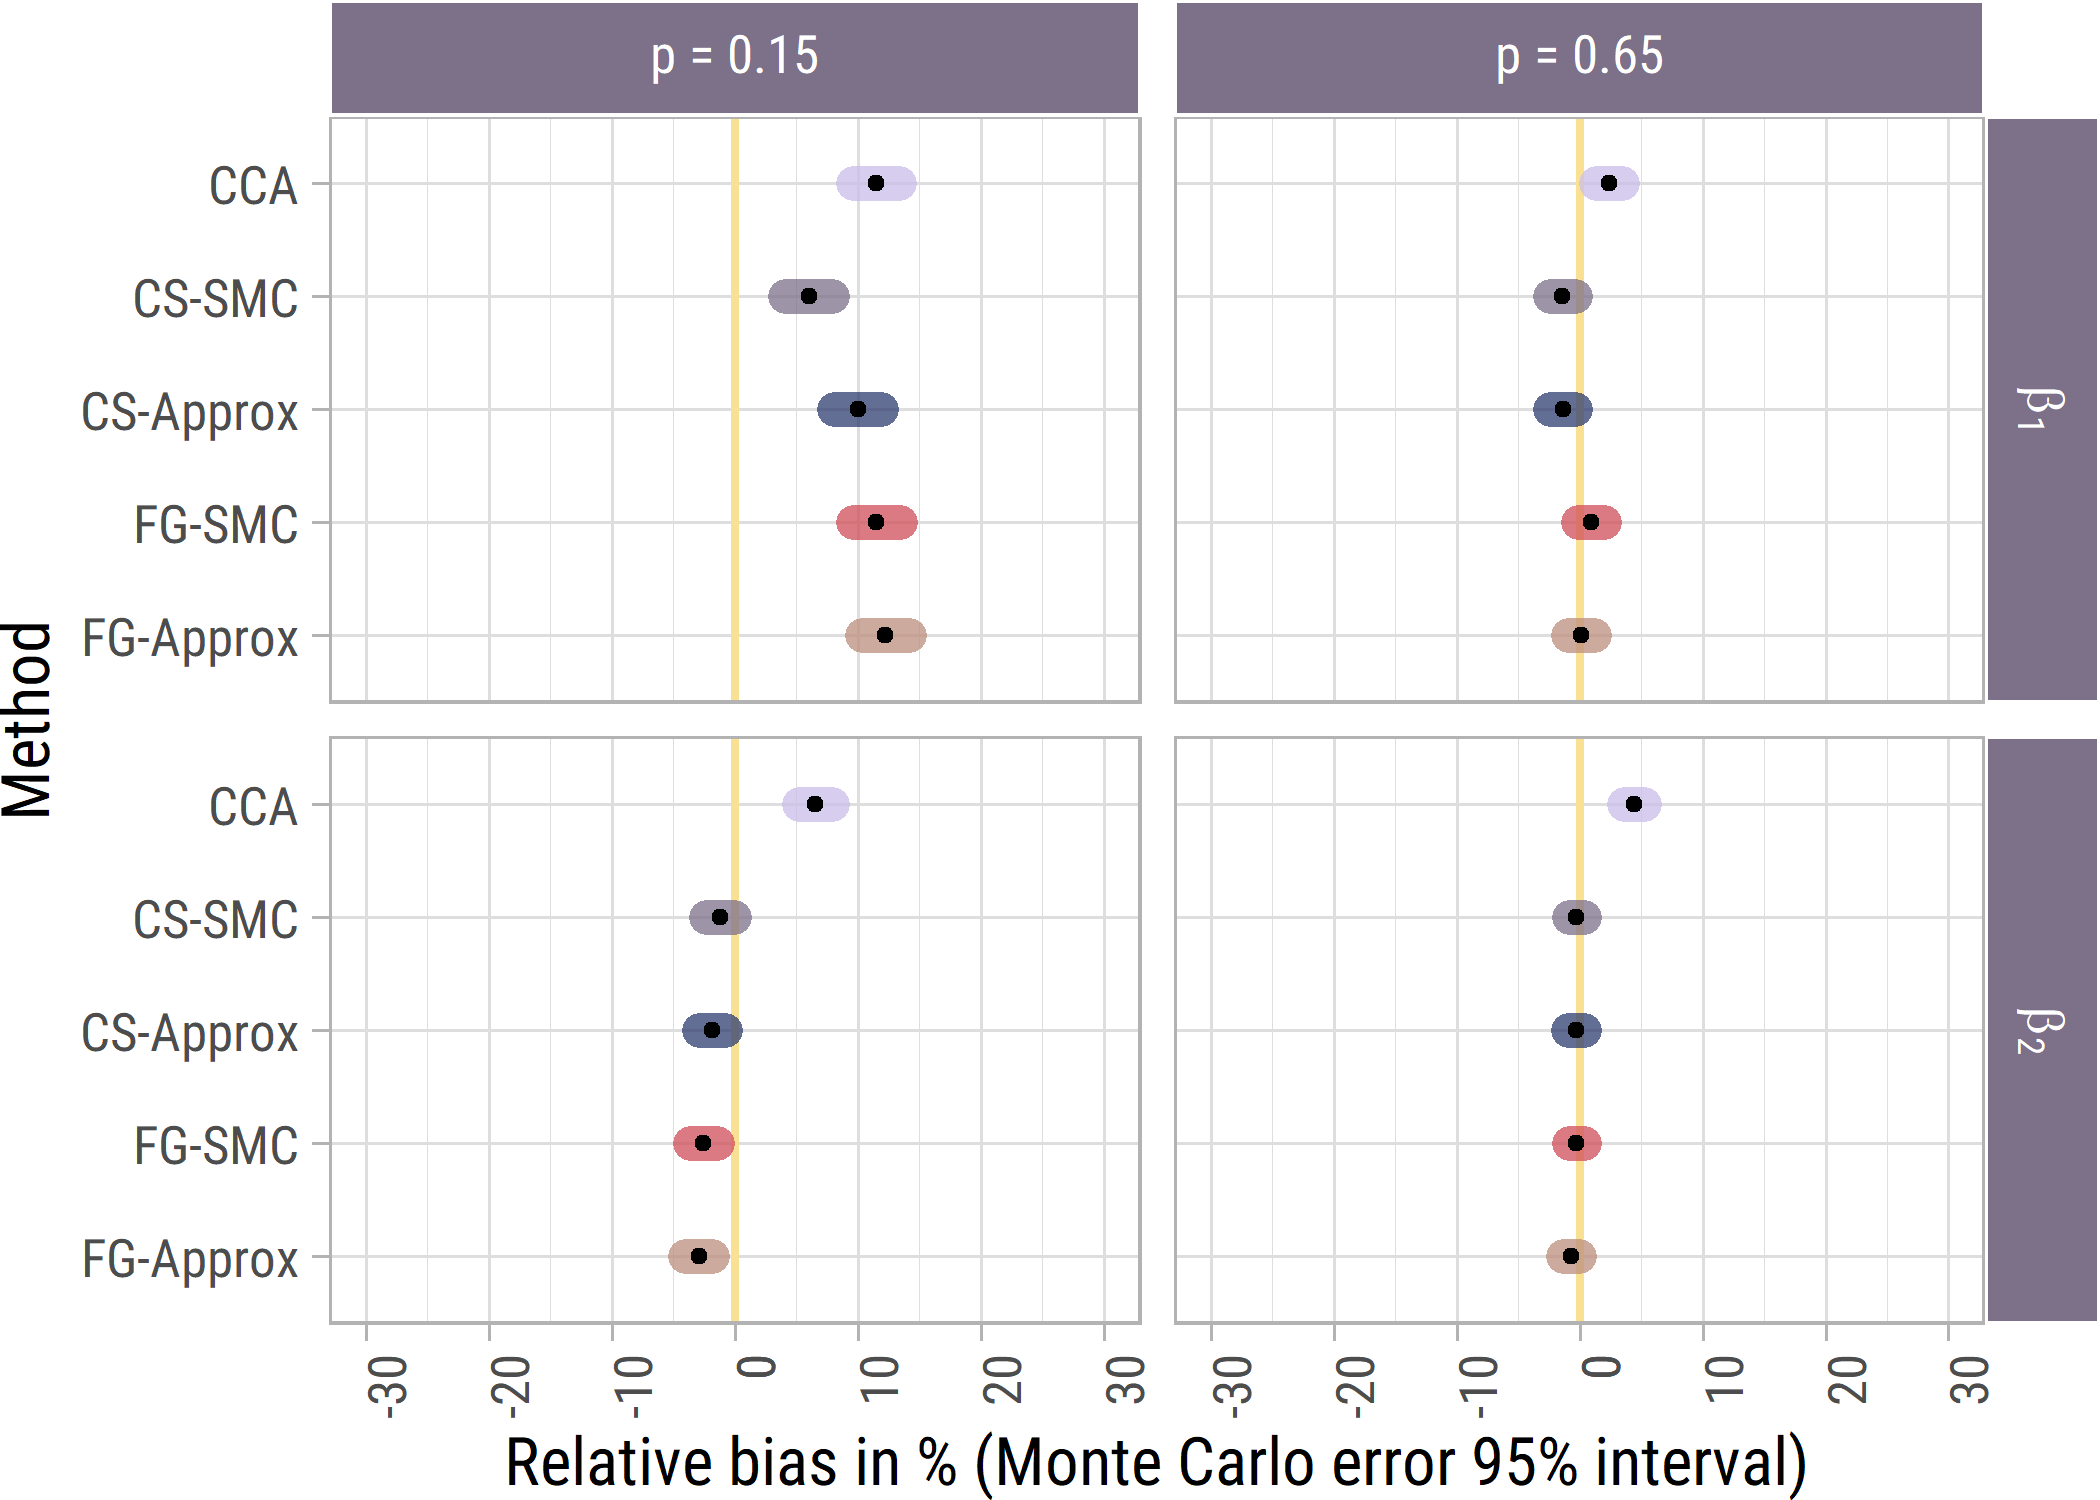
\includegraphics{figures/rel-bias-plots-mart-1.pdf}

\subsection{Supplementary simulations: covariate-dependent
censoring}\label{supplementary-simulations-covariate-dependent-censoring}

\newpage

\section{Applied data example}\label{applied-data-example}

\subsection{Data dictionary}\label{data-dictionary}

\begin{longtable}[t]{lc}

\caption{\label{tbl-data-dict}Data dictionary. CMV: cytomegalovirus;
HLA: human leukocyte antigen; HCT-CI: Hematopoietic stem cell
transplantation-comorbidity index; MF: myelofibrosis.}

\tabularnewline

\\
\toprule
Characteristic & N = 3,982\\
\midrule
Patient age (years) & 58 (52, 64)\\
Patient/donor CMV match & \\
\hspace{1em}Patient negative/Donor negative & 1,142 (30\%)\\
\hspace{1em}Other & 2,715 (70\%)\\
\hspace{1em}(Missing) & 125\\
Donor type & \\
\hspace{1em}HLA identical sibling & 1,183 (30\%)\\
\hspace{1em}Other & 2,795 (70\%)\\
\hspace{1em}(Missing) & 4\\
Hemoglobin (g/dL) & 9.10 (8.10, 10.40)\\
\hspace{1em}(Missing) & 1,873\\
HCT-CI risk category & \\
\hspace{1em}Low risk ($0$) & 1,674 (54\%)\\
\hspace{1em}Intermediate risk ($1-2$) & 743 (24\%)\\
\hspace{1em}High risk ($\geq 3$) & 674 (22\%)\\
\hspace{1em}(Missing) & 891\\
Interval diagnosis-transplantation (years) & 3 (1, 9)\\
Karnosfky performance score & \\
\hspace{1em}$\geq 90$ & 2,475 (66\%)\\
\hspace{1em}$80$ & 986 (26\%)\\
\hspace{1em}$\leq 70$ & 267 (7.2\%)\\
\hspace{1em}(Missing) & 254\\
Patient sex & \\
\hspace{1em}Female & 1,484 (37\%)\\
\hspace{1em}Male & 2,498 (63\%)\\
Peripheral blood (PB) blasts (\%) & 1.0 (0.0, 3.0)\\
\hspace{1em}(Missing) & 2,323\\
Conditioning & \\
\hspace{1em}Standard & 1,373 (35\%)\\
\hspace{1em}Reduced & 2,553 (65\%)\\
\hspace{1em}(Missing) & 56\\
Ruxolitinib given & \\
\hspace{1em}No & 1,832 (66\%)\\
\hspace{1em}Yes & 931 (34\%)\\
\hspace{1em}(Missing) & 1,219\\
Disease subclassification & \\
\hspace{1em}Primary MF & 2,912 (73\%)\\
\hspace{1em}Secondary MF & 1,070 (27\%)\\
Night sweats & \\
\hspace{1em}No & 1,256 (70\%)\\
\hspace{1em}Yes & 529 (30\%)\\
\hspace{1em}(Missing) & 2,197\\
T-cell depletion (in- or ev-vivo) & \\
\hspace{1em}No & 1,012 (26\%)\\
\hspace{1em}Yes & 2,905 (74\%)\\
\hspace{1em}(Missing) & 65\\
Cytogenetics & \\
\hspace{1em}Normal & 1,318 (59\%)\\
\hspace{1em}Abnormal & 910 (41\%)\\
\hspace{1em}(Missing) & 1,754\\
White blood cell count (WBC, x$10^9$/L) & 7 (4, 14)\\
\hspace{1em}(Missing) & 1,884\\
>10\% Weight loss prior to transplantation & \\
\hspace{1em}No & 1,329 (73\%)\\
\hspace{1em}Yes & 492 (27\%)\\
\hspace{1em}(Missing) & 2,161\\
Year of transplantation & 2,015.0 (2,012.0, 2,018.0)\\
\bottomrule
\multicolumn{2}{l}{\rule{0pt}{1em}\textsuperscript{1} Median (IQR); n (\%)}\\

\end{longtable}

\subsection{Non-parametric cumulative incidence
curves}\label{non-parametric-cumulative-incidence-curves}

\subsection{Pooled regression
coefficients}\label{pooled-regression-coefficients}

\begingroup\fontsize{9}{11}\selectfont

\begin{longtable}[t]{lrrr}

\caption{\label{tbl-pooled-coefs}Pooled log hazard ratios {[}log HR,
95\% confidence interval{]} for Fine--Gray model for relapse,
cause-specific Cox model relapse, and cause-specific Cox model for
non-relapse mortality (NRM).}

\tabularnewline

\\
\toprule
Term + method & Relapse subdist.~log HR & Relapse cause-spec.~log HR & NRM cause-spec.~log HR\\
\midrule
\endfirsthead
\caption[]{\textit{(continued)}}\\
\toprule
Term + method & Relapse subdist.~log HR & Relapse cause-spec.~log HR & NRM cause-spec.~log HR\\
\midrule
\endhead
\midrule
\multicolumn{4}{r@{}}{\textit{(continued \ldots)}}\\
\endfoot
\bottomrule
\endlastfoot
\addlinespace[0.3em]
\multicolumn{4}{l}{\textbf{Conditioning: reduced}}\\
\hspace{1em}CCA & 0.02 [-0.33, 0.36] & 0.01 [-0.33, 0.35] & 0 [-0.29, 0.28]\\
\hspace{1em}CS-SMC & 0.13 [-0.02, 0.28] & 0.1 [-0.05, 0.25] & -0.05 [-0.18, 0.07]\\
\hspace{1em}CS-Approx & 0.13 [-0.02, 0.28] & 0.1 [-0.05, 0.25] & -0.05 [-0.18, 0.07]\\
\hspace{1em}FG-SMC & 0.13 [-0.02, 0.28] & 0.1 [-0.05, 0.25] & -0.06 [-0.18, 0.07]\\
\hspace{1em}FG-Approx & 0.13 [-0.03, 0.28] & 0.1 [-0.06, 0.25] & -0.05 [-0.18, 0.07]\\
\addlinespace[0.3em]
\multicolumn{4}{l}{\textbf{CMV match: other}}\\
\hspace{1em}CCA & 0.04 [-0.31, 0.4] & 0.05 [-0.3, 0.41] & 0.09 [-0.19, 0.37]\\
\hspace{1em}CS-SMC & -0.1 [-0.26, 0.05] & -0.05 [-0.2, 0.11] & 0.22 [0.08, 0.36]\\
\hspace{1em}CS-Approx & -0.1 [-0.26, 0.05] & -0.05 [-0.2, 0.11] & 0.22 [0.08, 0.36]\\
\hspace{1em}FG-SMC & -0.1 [-0.26, 0.05] & -0.04 [-0.2, 0.11] & 0.22 [0.08, 0.36]\\
\hspace{1em}FG-Approx & -0.11 [-0.26, 0.05] & -0.05 [-0.2, 0.11] & 0.22 [0.08, 0.35]\\
\addlinespace[0.3em]
\multicolumn{4}{l}{\textbf{Cytogenetics: abnormal}}\\
\hspace{1em}CCA & 0.36 [0.04, 0.68] & 0.37 [0.05, 0.68] & -0.08 [-0.35, 0.19]\\
\hspace{1em}CS-SMC & 0.35 [0.15, 0.54] & 0.35 [0.16, 0.54] & -0.07 [-0.23, 0.1]\\
\hspace{1em}CS-Approx & 0.36 [0.17, 0.55] & 0.35 [0.16, 0.54] & -0.08 [-0.25, 0.08]\\
\hspace{1em}FG-SMC & 0.36 [0.17, 0.55] & 0.36 [0.17, 0.54] & -0.06 [-0.21, 0.08]\\
\hspace{1em}FG-Approx & 0.34 [0.17, 0.52] & 0.34 [0.17, 0.51] & -0.07 [-0.22, 0.08]\\
\addlinespace[0.3em]
\multicolumn{4}{l}{\textbf{Donor relation: other}}\\
\hspace{1em}CCA & 0.12 [-0.28, 0.52] & 0.2 [-0.2, 0.6] & 0.53 [0.18, 0.88]\\
\hspace{1em}CS-SMC & -0.26 [-0.41, -0.1] & -0.19 [-0.34, -0.03] & 0.35 [0.21, 0.5]\\
\hspace{1em}CS-Approx & -0.25 [-0.41, -0.1] & -0.18 [-0.34, -0.02] & 0.36 [0.21, 0.5]\\
\hspace{1em}FG-SMC & -0.26 [-0.41, -0.1] & -0.19 [-0.34, -0.03] & 0.35 [0.2, 0.49]\\
\hspace{1em}FG-Approx & -0.26 [-0.41, -0.1] & -0.19 [-0.34, -0.03] & 0.35 [0.2, 0.49]\\
\addlinespace[0.3em]
\multicolumn{4}{l}{\textbf{Hemoglobin (per $5$ g/dL)}}\\
\hspace{1em}CCA & -0.38 [-0.85, 0.09] & -0.39 [-0.85, 0.08] & -0.12 [-0.49, 0.25]\\
\hspace{1em}CS-SMC & -0.24 [-0.51, 0.03] & -0.3 [-0.58, -0.03] & -0.19 [-0.42, 0.04]\\
\hspace{1em}CS-Approx & -0.25 [-0.53, 0.02] & -0.32 [-0.59, -0.06] & -0.19 [-0.41, 0.02]\\
\hspace{1em}FG-SMC & -0.25 [-0.51, 0.02] & -0.29 [-0.56, -0.02] & -0.08 [-0.28, 0.11]\\
\hspace{1em}FG-Approx & -0.23 [-0.5, 0.04] & -0.27 [-0.54, 0] & -0.09 [-0.29, 0.11]\\
\addlinespace[0.3em]
\multicolumn{4}{l}{\textbf{HCT-CI ($1-2$)}}\\
\hspace{1em}CCA & -0.15 [-0.53, 0.22] & -0.04 [-0.42, 0.33] & 0.38 [0.08, 0.69]\\
\hspace{1em}CS-SMC & -0.22 [-0.42, -0.01] & -0.17 [-0.37, 0.03] & 0.15 [-0.02, 0.31]\\
\hspace{1em}CS-Approx & -0.19 [-0.38, 0.01] & -0.14 [-0.34, 0.06] & 0.15 [-0.01, 0.31]\\
\hspace{1em}FG-SMC & -0.22 [-0.42, -0.01] & -0.18 [-0.38, 0.02] & 0.12 [-0.04, 0.28]\\
\hspace{1em}FG-Approx & -0.19 [-0.38, 0.01] & -0.15 [-0.35, 0.04] & 0.11 [-0.05, 0.27]\\
\addlinespace[0.3em]
\multicolumn{4}{l}{\textbf{HCT-CI ($\geq 3$)}}\\
\hspace{1em}CCA & -0.27 [-0.7, 0.16] & -0.19 [-0.62, 0.23] & 0.4 [0.07, 0.73]\\
\hspace{1em}CS-SMC & -0.07 [-0.28, 0.14] & -0.01 [-0.21, 0.2] & 0.27 [0.1, 0.44]\\
\hspace{1em}CS-Approx & -0.08 [-0.28, 0.13] & -0.02 [-0.22, 0.18] & 0.26 [0.1, 0.43]\\
\hspace{1em}FG-SMC & -0.06 [-0.27, 0.14] & -0.02 [-0.22, 0.19] & 0.21 [0.05, 0.37]\\
\hspace{1em}FG-Approx & -0.08 [-0.28, 0.11] & -0.04 [-0.23, 0.16] & 0.21 [0.05, 0.38]\\
\addlinespace[0.3em]
\multicolumn{4}{l}{\textbf{Interval diagnosis to alloHCT (decades)}}\\
\hspace{1em}CCA & 0.01 [-0.24, 0.26] & 0 [-0.25, 0.26] & -0.03 [-0.25, 0.19]\\
\hspace{1em}CS-SMC & -0.02 [-0.14, 0.09] & -0.02 [-0.14, 0.1] & 0.05 [-0.05, 0.15]\\
\hspace{1em}CS-Approx & -0.03 [-0.14, 0.09] & -0.02 [-0.14, 0.1] & 0.05 [-0.05, 0.15]\\
\hspace{1em}FG-SMC & -0.02 [-0.14, 0.09] & -0.02 [-0.13, 0.1] & 0.05 [-0.05, 0.15]\\
\hspace{1em}FG-Approx & -0.02 [-0.14, 0.09] & -0.02 [-0.14, 0.1] & 0.05 [-0.05, 0.15]\\
\addlinespace[0.3em]
\multicolumn{4}{l}{\textbf{Karnofsky ($80$)}}\\
\hspace{1em}CCA & -0.09 [-0.48, 0.31] & -0.08 [-0.48, 0.31] & 0.04 [-0.27, 0.34]\\
\hspace{1em}CS-SMC & 0.07 [-0.1, 0.24] & 0.12 [-0.05, 0.28] & 0.17 [0.03, 0.31]\\
\hspace{1em}CS-Approx & 0.06 [-0.1, 0.23] & 0.1 [-0.06, 0.27] & 0.15 [0.01, 0.29]\\
\hspace{1em}FG-SMC & 0.07 [-0.09, 0.24] & 0.12 [-0.05, 0.29] & 0.17 [0.03, 0.31]\\
\hspace{1em}FG-Approx & 0.07 [-0.1, 0.24] & 0.12 [-0.06, 0.29] & 0.17 [0.03, 0.31]\\
\addlinespace[0.3em]
\multicolumn{4}{l}{\textbf{Karnofsky ($\leq 70$)}}\\
\hspace{1em}CCA & 0.63 [0.15, 1.11] & 0.79 [0.3, 1.28] & 0.33 [-0.13, 0.79]\\
\hspace{1em}CS-SMC & 0.44 [0.19, 0.69] & 0.55 [0.3, 0.81] & 0.31 [0.08, 0.53]\\
\hspace{1em}CS-Approx & 0.42 [0.17, 0.67] & 0.51 [0.26, 0.76] & 0.26 [0.04, 0.49]\\
\hspace{1em}FG-SMC & 0.44 [0.19, 0.7] & 0.55 [0.29, 0.81] & 0.32 [0.09, 0.54]\\
\hspace{1em}FG-Approx & 0.43 [0.17, 0.68] & 0.53 [0.28, 0.78] & 0.31 [0.08, 0.53]\\
\addlinespace[0.3em]
\multicolumn{4}{l}{\textbf{Disease subclassification: secondary MF}}\\
\hspace{1em}CCA & -0.05 [-0.45, 0.35] & -0.02 [-0.42, 0.38] & 0.07 [-0.27, 0.41]\\
\hspace{1em}CS-SMC & 0.01 [-0.17, 0.19] & 0.01 [-0.17, 0.19] & 0 [-0.16, 0.15]\\
\hspace{1em}CS-Approx & 0 [-0.18, 0.18] & 0 [-0.18, 0.19] & 0 [-0.16, 0.15]\\
\hspace{1em}FG-SMC & 0 [-0.18, 0.18] & 0 [-0.18, 0.18] & -0.01 [-0.16, 0.15]\\
\hspace{1em}FG-Approx & 0 [-0.18, 0.18] & 0 [-0.18, 0.18] & -0.01 [-0.16, 0.15]\\
\addlinespace[0.3em]
\multicolumn{4}{l}{\textbf{Night sweats: yes}}\\
\hspace{1em}CCA & -0.33 [-0.7, 0.04] & -0.4 [-0.77, -0.02] & -0.02 [-0.32, 0.27]\\
\hspace{1em}CS-SMC & -0.18 [-0.41, 0.05] & -0.2 [-0.44, 0.03] & -0.02 [-0.23, 0.19]\\
\hspace{1em}CS-Approx & -0.12 [-0.36, 0.13] & -0.14 [-0.38, 0.1] & 0.03 [-0.19, 0.24]\\
\hspace{1em}FG-SMC & -0.17 [-0.4, 0.07] & -0.18 [-0.41, 0.05] & 0.01 [-0.16, 0.19]\\
\hspace{1em}FG-Approx & -0.16 [-0.4, 0.07] & -0.18 [-0.42, 0.05] & 0 [-0.17, 0.18]\\
\addlinespace[0.3em]
\multicolumn{4}{l}{\textbf{Patient age (decades)}}\\
\hspace{1em}CCA & 0.1 [-0.09, 0.28] & 0.13 [-0.06, 0.32] & 0.13 [-0.02, 0.28]\\
\hspace{1em}CS-SMC & -0.03 [-0.12, 0.05] & 0.01 [-0.08, 0.09] & 0.21 [0.14, 0.29]\\
\hspace{1em}CS-Approx & -0.03 [-0.12, 0.05] & 0.01 [-0.08, 0.09] & 0.21 [0.14, 0.29]\\
\hspace{1em}FG-SMC & -0.04 [-0.12, 0.05] & 0.01 [-0.08, 0.09] & 0.22 [0.15, 0.3]\\
\hspace{1em}FG-Approx & -0.03 [-0.12, 0.05] & 0.01 [-0.08, 0.09] & 0.22 [0.15, 0.3]\\
\addlinespace[0.3em]
\multicolumn{4}{l}{\textbf{Patient sex: male}}\\
\hspace{1em}CCA & -0.24 [-0.56, 0.09] & -0.18 [-0.51, 0.15] & 0.39 [0.11, 0.68]\\
\hspace{1em}CS-SMC & -0.1 [-0.24, 0.05] & -0.06 [-0.21, 0.09] & 0.18 [0.05, 0.31]\\
\hspace{1em}CS-Approx & -0.1 [-0.24, 0.05] & -0.06 [-0.21, 0.09] & 0.18 [0.05, 0.31]\\
\hspace{1em}FG-SMC & -0.09 [-0.24, 0.05] & -0.06 [-0.2, 0.09] & 0.18 [0.05, 0.31]\\
\hspace{1em}FG-Approx & -0.1 [-0.24, 0.05] & -0.06 [-0.21, 0.08] & 0.18 [0.05, 0.31]\\
\addlinespace[0.3em]
\multicolumn{4}{l}{\textbf{PB Blasts (per $5$\%)}}\\
\hspace{1em}CCA & 0.16 [-0.04, 0.36] & 0.17 [-0.02, 0.37] & 0 [-0.18, 0.18]\\
\hspace{1em}CS-SMC & 0.18 [0.05, 0.31] & 0.18 [0.05, 0.31] & 0.01 [-0.12, 0.13]\\
\hspace{1em}CS-Approx & 0.19 [0.07, 0.31] & 0.19 [0.07, 0.32] & 0.01 [-0.12, 0.13]\\
\hspace{1em}FG-SMC & 0.17 [0.04, 0.3] & 0.17 [0.05, 0.3] & -0.01 [-0.12, 0.1]\\
\hspace{1em}FG-Approx & 0.18 [0.05, 0.32] & 0.18 [0.05, 0.31] & -0.02 [-0.12, 0.09]\\
\addlinespace[0.3em]
\multicolumn{4}{l}{\textbf{Ruxolitinib given: yes}}\\
\hspace{1em}CCA & 0.08 [-0.26, 0.43] & 0.08 [-0.26, 0.43] & -0.05 [-0.33, 0.23]\\
\hspace{1em}CS-SMC & -0.02 [-0.2, 0.17] & -0.03 [-0.22, 0.16] & -0.06 [-0.21, 0.1]\\
\hspace{1em}CS-Approx & 0.01 [-0.19, 0.2] & -0.01 [-0.2, 0.18] & -0.05 [-0.21, 0.11]\\
\hspace{1em}FG-SMC & -0.02 [-0.21, 0.17] & -0.03 [-0.22, 0.16] & -0.04 [-0.19, 0.11]\\
\hspace{1em}FG-Approx & 0 [-0.19, 0.18] & -0.01 [-0.2, 0.17] & -0.04 [-0.19, 0.11]\\
\addlinespace[0.3em]
\multicolumn{4}{l}{\textbf{T-cell depletion: yes}}\\
\hspace{1em}CCA & 0.2 [-0.21, 0.62] & 0.16 [-0.25, 0.58] & -0.23 [-0.54, 0.08]\\
\hspace{1em}CS-SMC & 0.3 [0.13, 0.48] & 0.26 [0.09, 0.44] & -0.18 [-0.32, -0.04]\\
\hspace{1em}CS-Approx & 0.3 [0.12, 0.48] & 0.26 [0.08, 0.43] & -0.19 [-0.33, -0.05]\\
\hspace{1em}FG-SMC & 0.31 [0.13, 0.48] & 0.26 [0.09, 0.44] & -0.18 [-0.31, -0.04]\\
\hspace{1em}FG-Approx & 0.31 [0.13, 0.48] & 0.26 [0.09, 0.44] & -0.18 [-0.32, -0.04]\\
\addlinespace[0.3em]
\multicolumn{4}{l}{\textbf{WBC count (log)}}\\
\hspace{1em}CCA & 0.17 [0.02, 0.33] & 0.17 [0.01, 0.33] & 0.02 [-0.12, 0.15]\\
\hspace{1em}CS-SMC & 0.17 [0.09, 0.26] & 0.18 [0.09, 0.27] & 0 [-0.07, 0.07]\\
\hspace{1em}CS-Approx & 0.17 [0.08, 0.26] & 0.17 [0.09, 0.26] & 0 [-0.08, 0.07]\\
\hspace{1em}FG-SMC & 0.17 [0.09, 0.26] & 0.18 [0.09, 0.26] & -0.01 [-0.07, 0.05]\\
\hspace{1em}FG-Approx & 0.17 [0.1, 0.25] & 0.18 [0.1, 0.26] & -0.01 [-0.08, 0.05]\\
\addlinespace[0.3em]
\multicolumn{4}{l}{\textbf{Weight loss: yes}}\\
\hspace{1em}CCA & 0 [-0.37, 0.38] & 0.05 [-0.33, 0.43] & 0.17 [-0.13, 0.48]\\
\hspace{1em}CS-SMC & 0.23 [-0.03, 0.49] & 0.27 [0.01, 0.53] & 0.16 [-0.05, 0.36]\\
\hspace{1em}CS-Approx & 0.24 [0, 0.47] & 0.28 [0.04, 0.51] & 0.16 [-0.05, 0.36]\\
\hspace{1em}FG-SMC & 0.23 [-0.01, 0.47] & 0.24 [0.01, 0.48] & 0.06 [-0.12, 0.24]\\
\hspace{1em}FG-Approx & 0.24 [0, 0.48] & 0.26 [0.02, 0.49] & 0.06 [-0.14, 0.26]\\
\addlinespace[0.3em]
\multicolumn{4}{l}{\textbf{Year of alloHCT (decades)}}\\
\hspace{1em}CCA & -0.36 [-0.99, 0.26] & -0.41 [-1.04, 0.23] & -0.15 [-0.67, 0.37]\\
\hspace{1em}CS-SMC & -0.08 [-0.34, 0.18] & -0.11 [-0.37, 0.15] & -0.24 [-0.46, -0.02]\\
\hspace{1em}CS-Approx & -0.09 [-0.35, 0.17] & -0.12 [-0.38, 0.14] & -0.24 [-0.46, -0.02]\\
\hspace{1em}FG-SMC & -0.08 [-0.34, 0.17] & -0.12 [-0.37, 0.14] & -0.24 [-0.46, -0.03]\\
\hspace{1em}FG-Approx & -0.08 [-0.34, 0.17] & -0.11 [-0.37, 0.14] & -0.24 [-0.46, -0.03]\\*

\end{longtable}

\endgroup{}




\end{document}
